\section{Drive a device with an NPN BJT}
This exercise has a $5V$ logic output (the $V_{ter}$ in Figure \ref{lab3_ex2_de}) that can source up to $10mA$ of current without a severe voltage drop and stand a maximum current of $20mA$. If the logic terminal sources a current larger than $20mA$, it would be damaged. Or, if it sources a current larger than $10mA$, the $V_{ter}$ voltage will drop to less than $4V$. We should avoid this drop in many cases.  However, this logic terminal has to be used to drive an electrical component with an equivalent internal resistance of 5 ohms (the LOAD in Figure \ref{lab3_ex2_de}) and requires a current of at least $300mA$ and not exceeding $500mA$ to function normally.
Given that we have an NPN transistor with the current gain $\beta$ equals $100$, the maximum $I_C$ current is $400mA$, and the barrier potential at the BE junction is $V_{BE} = 0.7V$, select a resistor available in the market to replace the resistor $R_B$ revealed in Figure \ref{lab3_ex2_de}. to make the circuit function well. After that, perform a simulation to double-check your selection.

\begin{figure}[h]
    \centering
    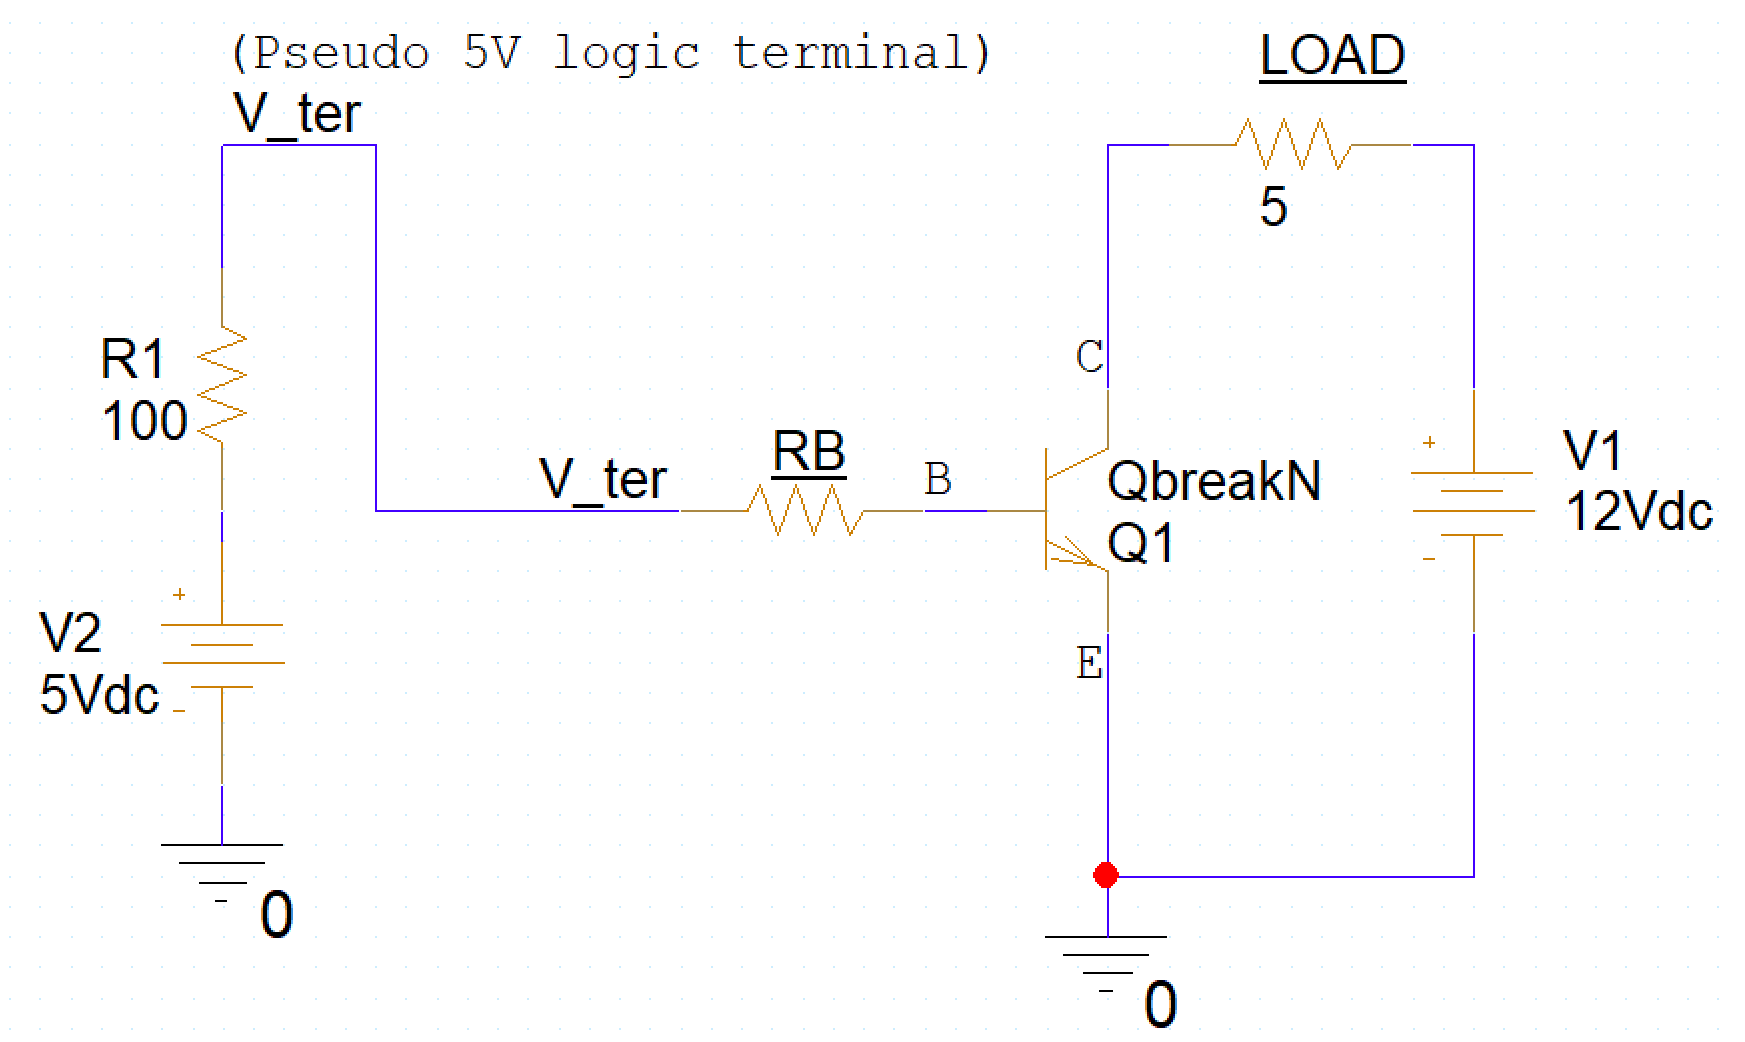
\includegraphics[width=12cm]{graphics/ex4/f1.png}
    \caption{Select a resistor available in the market for \(R_B\)}
    \label{lab3_ex2_de}
\end{figure}

\subsection{Theory calculations}

\textbf{Notes:}

\textit{Explanations, formulas, and equations are expected rather than only results.}

Ta có $I_C=\beta I_B$

Theo giới hạn của TẢI và bóng bán dẫn, ta có:
\begin{align*}
    300 \, \text{mA} \, (\text{min}) <\, &I_C < 400 \, \text{mA} \, (\text{max})\\
    3 \, \text{mA} \, (\text{min}) <\, &I_B < 4 \, \text{mA} \, (\text{max})
\end{align*}

Với \( I_B (\text{min}) = 3 \, \text{mA} \) ta có:
\[
R_B (\text{max}) = \frac{V_2 - I_BR_1 - V_{BE}}{I_B} =1333.3 \, \Omega
\]
Với \( I_B (\text{max}) = 4 \, \text{mA} \) ta có:
\[
R_B (\text{min}) = \frac{V_2 - I_BR_1 - V_{BE}}{I_B} = 975 \, \Omega
\]
Vậy:
\[
975 \, \Omega \, (\text{min}) < R_B < 1333.3 \, \Omega \, (\text{max})
\]
$R_B$ được chọn là: \( 1100 \, \Omega \)

\subsection{Simulation}

Your image goes here

$R_B (min) = 975$
\begin{figure}[h]
    \centering
    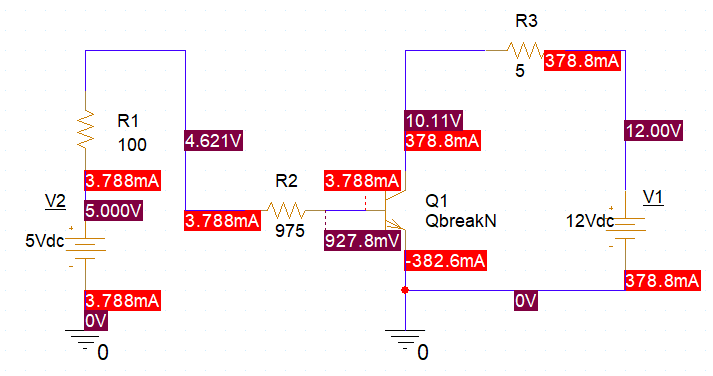
\includegraphics[width=12cm]{graphics/ex4/f2.PNG}
\end{figure}
\newpage
$R_B (max) = 1333.3$
\begin{figure}[h]
    \centering
    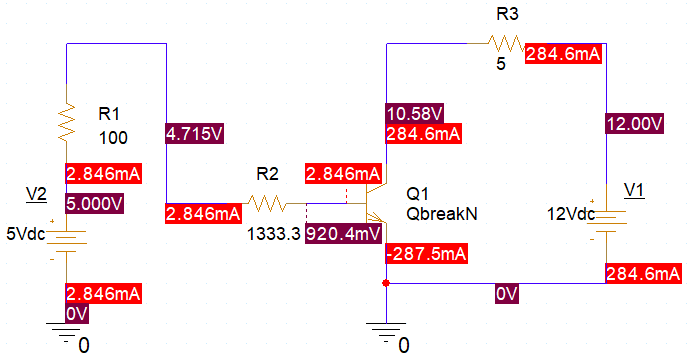
\includegraphics[width=12cm]{graphics/ex4/f3.PNG}
\end{figure}

$R_B (selected) = 1100$
\begin{figure}[h]
    \centering
    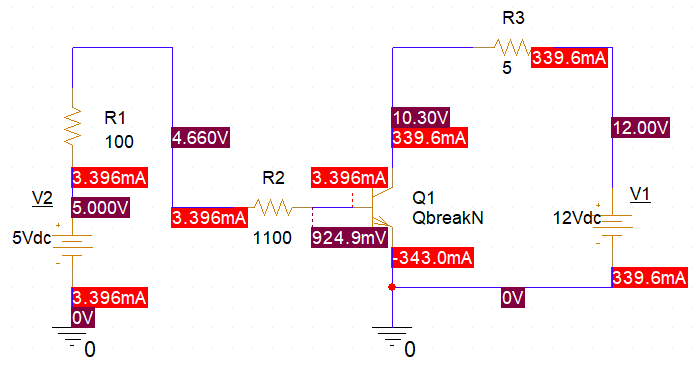
\includegraphics[width=12cm]{graphics/ex4/f4.PNG}
\end{figure}
\subsection{Compare}

\begin{center}
    \begin{tabular}{l|l|l|l|l|l|l|l|}
    \cline{2-8}
                                     & & \multicolumn{3}{c|}{\textbf{Theory}} & \multicolumn{3}{c|}{\textbf{PSpice}} \\ \cline{2-8} 
                                     &$R_B$ & $V_{BE}$              & $I_B$              & $I_C$              & $V_{BE}$              & $I_B$              & $I_C$             \\ \hline
     \multicolumn{1}{|l|}{$R_B(min)$} &\( 975 \, \Omega \) & \( 0.7 \, \text{V} \) & \( 4 \, \text{mA} \) & \( 400 \, \text{mA} \) & \( 0.928 \, \text{V} \) & \( 3.788 \, \text{mA} \) & \( 378.8 \, \text{mA} \) \\ \hline
    \multicolumn{1}{|l|}{$R_B(max)$}  &\( 1333.3 \, \Omega \) & \( 0.7 \, \text{V} \) & \( 3 \, \text{mA} \) & \( 300 \, \text{mA} \) & \( 0.920 \, \text{V} \) & \( 2.846 \, \text{mA} \) & \( 284.6 \, \text{mA} \) \\ \hline
        \multicolumn{1}{|l|}{$R_B(selected)$}  &\( 1100 \, \Omega \) & \( 0.7 \, \text{V} \) & \( 3.58 \, \text{mA} \) & \( 358 \, \text{mA} \) & \( 0.925 \, \text{V} \) & \( 3.396 \, \text{mA} \) & \( 339.6 \, \text{mA} \) \\ \hline

    \end{tabular}
\end{center}